% !TeX program = xelatex
\documentclass[aspectratio=169,10pt,xcolor=dvipsnames]{beamer}
\usetheme{SimplePlus}
\usepackage{ctex}
\usepackage{amsmath,amssymb,mathtools}
\usepackage{booktabs}
\usepackage{graphicx}
\usepackage{hyperref}
\usepackage{tikz}
\usetikzlibrary{arrows.meta,positioning,calc,fit}
\setbeamertemplate{navigation symbols}{}
\setbeamertemplate{footline}[frame number]

\definecolor{cbBlue}{HTML}{2F6B9A}
\definecolor{cbTeal}{HTML}{2A7F72}
\definecolor{cbOrange}{HTML}{C86F2D}
\definecolor{cbGreen}{HTML}{4D7C5D}
\definecolor{ink}{HTML}{17324D}
\definecolor{muted}{HTML}{60758A}
\newcommand{\src}[1]{\vspace{1pt}\par{\scriptsize\color{muted}\raggedleft\texttt{\detokenize{#1}}\par}}
\newcommand{\blue}[1]{\textcolor{cbBlue}{#1}}
\newcommand{\teal}[1]{\textcolor{cbTeal}{#1}}
\newcommand{\orange}[1]{\textcolor{cbOrange}{#1}}
\newcommand{\green}[1]{\textcolor{cbGreen}{#1}}
\newcommand{\ns}{\mathrm{ns}}
\newcommand{\B}{\mathrm{B}}
\newcommand{\KV}{\mathrm{KV}}

\logo{\begin{tikzpicture}[remember picture,overlay]\node[anchor=north east,inner sep=2.5pt] at (current page.north east){
\includegraphics[width=1cm]{seu_logo.png}};\end{tikzpicture}}

\title{LLMServingSim 2.0 底层机制与时延模型}
\subtitle{从 vLLM 风格调度到 Chakra / ASTRA-Sim 周期级仿真}
\author{汇报人}
\institute{东南大学}
\date{\today}

\begin{document}

\begin{frame}\titlepage\end{frame}

\begin{frame}{目录}
  \tableofcontents
\end{frame}

\section{为什么需要周期级模型}
\begin{frame}[plain]
  \begin{tikzpicture}[remember picture,overlay]
    \node[inner sep=0pt] at (current page.center) {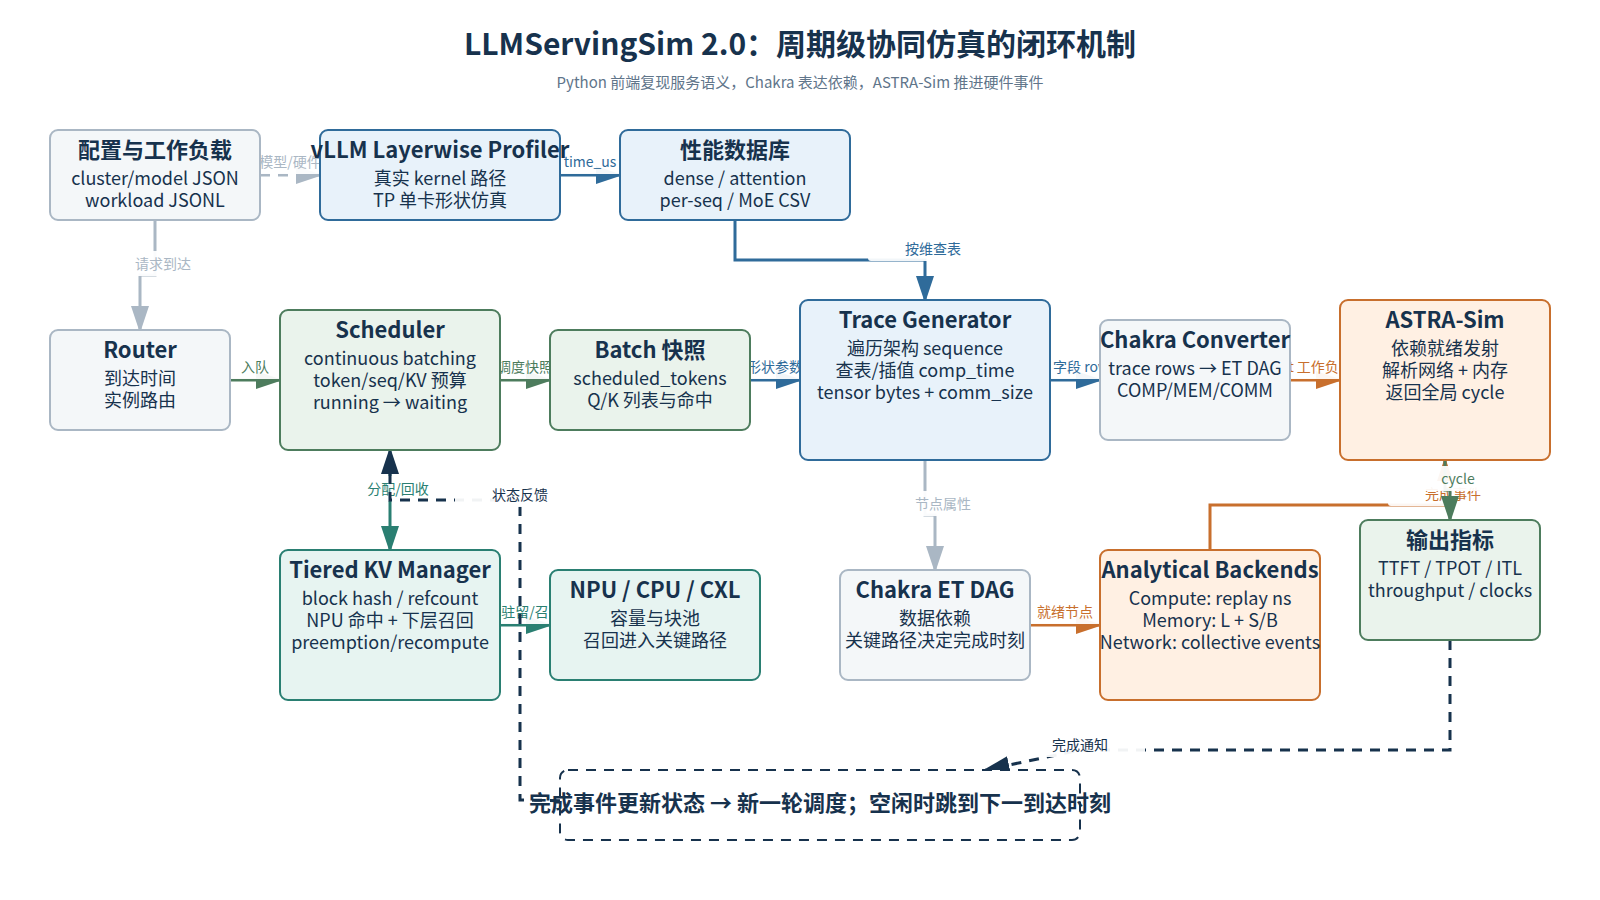
\includegraphics[width=\paperwidth,height=\paperheight]{figures/system-mechanism.png}};
  \end{tikzpicture}
\end{frame}

\begin{frame}{仿真对象：一次迭代是一个可依赖的 DAG}
  \begin{columns}[T]
    \column{0.48\textwidth}
    \textbf{前端状态}
    \begin{itemize}
      \item Router：按到达时间与实例负载分发
      \item Scheduler：running 优先，受 token / seq / KV 预算约束
      \item Batch：记录本轮实际 scheduled tokens 与 KV 命中
      \item Trace：把 batch 形状映射到每层节点
    \end{itemize}
    \column{0.48\textwidth}
    \textbf{后端事件}
    \begin{itemize}
      \item COMP：回放 profile 中的 kernel duration
      \item MEM：按 memory tier 的带宽与延迟发事件
      \item COMM：把 collective 拆成可调度的通信 phase
      \item 完成时刻：所有依赖与资源约束同时满足
    \end{itemize}
  \end{columns}
  \vfill
  \begin{block}{建模边界}
    调度、KV 与 trace 在 Python 中决定工作内容；Chakra 只表达依赖，ASTRA-Sim 推进硬件时钟。
  \end{block}
  \src{serving/core/scheduler.py:90--131; astra-sim/astra-sim/workload/Workload.cc:115--190}
\end{frame}

\begin{frame}{统一输入：batch 形状，而不是“prefill/decode”标签}
  \begin{equation*}
    x=\bigl(T,\;N_{\rm seq},\;p_c,\;k_p,\;N_d,\;k_d^{\rm mean},\;k_d^{\rm max},\;TP,PP,EP\bigr)
  \end{equation*}
  \begin{columns}[T]
    \column{0.48\textwidth}
    \begin{itemize}
      \item $T=\sum_i n_i$：本轮真正计算的 token 数
      \item $n_i>1$：prefill chunk；$n_i=1$：decode
      \item $p_c=\sum$ prefill query，$k_p=\sum$ prefill history
    \end{itemize}
    \column{0.48\textwidth}
    \begin{itemize}
      \item $N_d$：decode request 数量
      \item $k_d^{\rm mean}=\lfloor\sum k_i/N_d\rfloor$
      \item 非均匀 decode 额外使用 $k_d^{\rm max},k_d^{\rm min}$
    \end{itemize}
  \end{columns}
  \vfill
  \begin{alertblock}{关键语义}
    恢复/重算仍按本轮 scheduled token 数分类；不能从 $num\_computed\_tokens$ 推断序列长度。
  \end{alertblock}
  \src{serving/core/scheduler.py:238--250, 272--338; serving/core/trace_generator.py:938--975}
\end{frame}

\section{系统执行机制}
\begin{frame}{调度：先服务 running，再尝试 admission}
  \begin{tikzpicture}[x=1cm,y=1cm,box/.style={draw,rounded corners=2pt,minimum height=0.7cm,text width=3.3cm,align=center,font=\small},arr/.style={-{Stealth},thick}]
    \node[box,fill=cbGreen!12,draw=cbGreen] (r) at (0,0) {Running\quad Phase A};
    \node[box,fill=cbOrange!12,draw=cbOrange] (p) at (4.6,0) {KV 不足？\quad tail preempt};
    \node[box,fill=cbBlue!12,draw=cbBlue] (w) at (9.2,0) {Waiting\quad Phase B};
    \node[box,fill=gray!10,draw=ink] (b) at (4.6,-1.55) {Build Batch\quad advance at schedule time};
    \draw[arr] (r)--node[above,font=\scriptsize]{budget consumed}(p);
    \draw[arr] (p)--node[above,font=\scriptsize]{no preemption}(w);
    \draw[arr] (w)--(b);
    \draw[arr,dashed] (p.south) |- (b.east);
  \end{tikzpicture}
  \vspace{7pt}
  \begin{equation*}
    n_i^{\rm new}=\min\!\left(\operatorname{threshold}(L_i-num\_computed_i),\;B_{\rm token}\right)
  \end{equation*}
  \begin{center}\small\orange{发生 preemption 的 step 跳过 waiting admission，避免“抢占 → 立即回填 → 再抢占”的震荡。}\end{center}
  \src{serving/core/scheduler.py:90--131, 133--236}
\end{frame}

\begin{frame}{KV 容量：静态权重与分页 KV 的分账}
  \begin{equation*}
    \boxed{\;C_{\KV}=\left\lfloor\frac{u\,M_{\rm NPU}-W}{B_{\rm block}}\right\rfloor B_{\rm block}\;},
    \qquad
    N_{\rm block}=\left\lfloor\frac{uM_{\rm NPU}-W}{B_{\rm block}}\right\rfloor
  \end{equation*}
  \begin{itemize}
    \item $u$：\texttt{\detokenize{npu_memory_utilization}}；$W$：单 NPU 保守权重上界
    \item $B_{\rm block}=b_{\rm tok}\cdot b_{\KV/token/rank}$，按 block 分配
    \item vLLM 会额外扣 activation peak / CUDA context；本模拟器没有建模，因此容量是同利用率下的上界
  \end{itemize}
  \begin{block}{容量什么时候影响结果？}
    只有工作集触顶才会触发 preemption、重算或下层召回；未触顶时容量不会直接改变 kernel duration。
  \end{block}
  \src{serving/core/memory_model.py:73--107; serving/core/kv_cache_manager.py:216--240}
\end{frame}

\begin{frame}{KV 字节公式：GQA、层数、TP 与 FP8}
  \begin{equation*}
    H_{\KV}=h_{\KV}d_{\rm head},\qquad
    b_{\KV}=\begin{cases}1,&\text{fp8 KV cache}\\ b_{\rm weight},&\text{otherwise}\end{cases}
  \end{equation*}
  \begin{equation*}
    \boxed{\;B_{\KV}(L,\text{per rank})
    =\frac{2H_{\KV}L\,N_{\rm layer}\,b_{\KV}}{N_{\rm NPU}}\;}
  \end{equation*}
  \begin{columns}[T]
    \column{0.48\textwidth}
    \textbf{含义}
    \begin{itemize}
      \item $2$：K 与 V
      \item $H_{\KV}$：KV heads × head dimension
      \item $N_{\rm layer}$：每层都保存 KV
    \end{itemize}
    \column{0.48\textwidth}
    \textbf{结果}
    \begin{itemize}
      \item GQA 使 $h_{\KV}<h_q$，KV 显著小于 QKV activation
      \item FP8 KV 直接将每元素从 2 bytes 降为 1 byte
      \item TP 只改变每 rank 持有的 shard
    \end{itemize}
  \end{columns}
  \src{serving/core/memory_model.py:48--55, 209--235}
\end{frame}

\begin{frame}{层级 KV：命中、召回与写回的时间语义}
  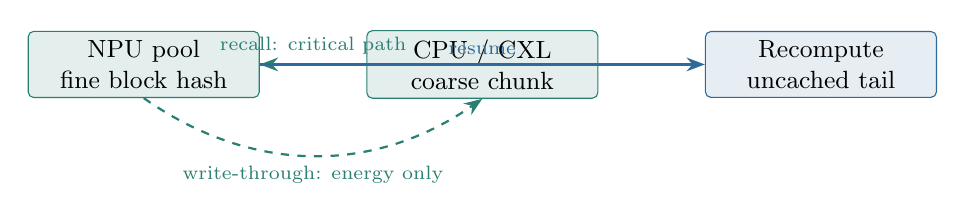
\begin{tikzpicture}[x=1cm,y=1cm,box/.style={draw,rounded corners=2pt,minimum height=0.8cm,text width=2.7cm,align=center,font=\small},arr/.style={-{Stealth},thick}]
    \node[box,fill=cbTeal!13,draw=cbTeal] (n) at (0,0) {NPU pool\\fine block hash};
    \node[box,fill=cbTeal!13,draw=cbTeal] (c) at (4.3,0) {CPU / CXL\\coarse chunk};
    \node[box,fill=cbBlue!12,draw=cbBlue] (x) at (8.6,0) {Recompute\\uncached tail};
    \draw[arr,cbTeal] (c)--node[above,font=\scriptsize]{recall: critical path}(n);
    \draw[arr,cbBlue] (n)--node[above,font=\scriptsize]{resume}(x);
    \draw[arr,dashed,cbTeal] (n.south) to[bend right=35] node[below,font=\scriptsize]{write-through: energy only}(c.south);
  \end{tikzpicture}
  \vspace{8pt}
  \begin{equation*}
    B_{\rm recall}=N_{\rm coarse\ blocks}\cdot B_{\rm coarse\ block},\qquad
    B_{\rm write}=N_{\rm newly\ full\ coarse\ blocks}\cdot B_{\rm coarse\ block}
  \end{equation*}
  \begin{center}\small\teal{free block 保留 hash；因此 preemption 后可以恢复仍驻留的最长前缀。}\end{center}
  \src{serving/core/kv_cache_manager.py:128--195, 297--355}
\end{frame}

\section{计算时延模型}
\begin{frame}[plain]
  \begin{tikzpicture}[remember picture,overlay]
    \node[inner sep=0pt] at (current page.center) {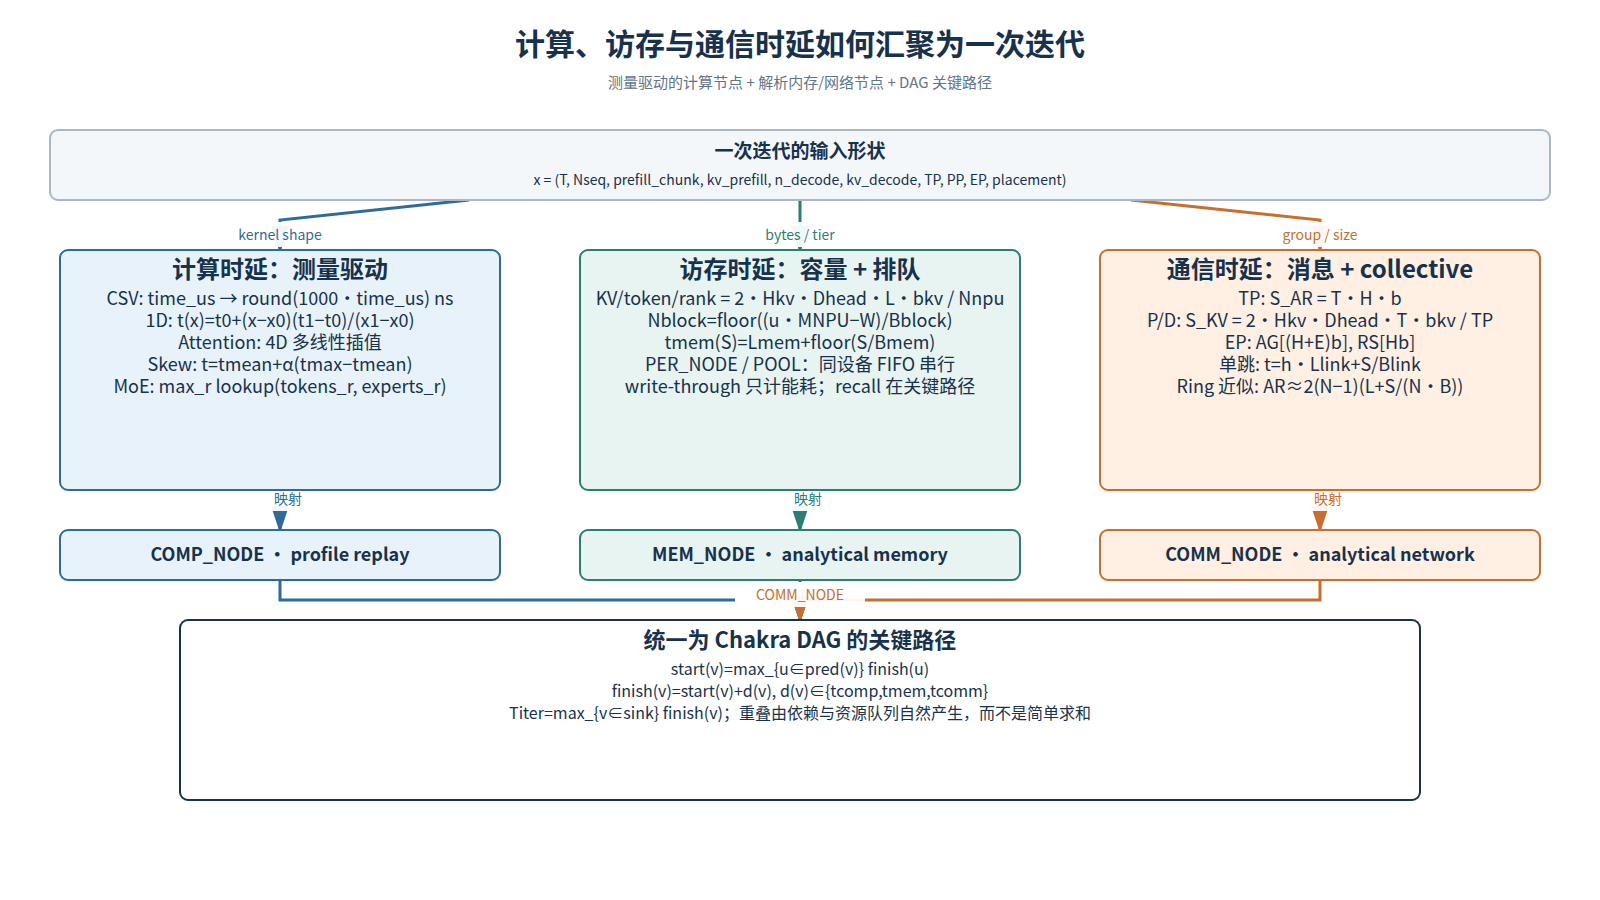
\includegraphics[width=\paperwidth,height=\paperheight]{figures/latency-model.png}};
  \end{tikzpicture}
\end{frame}

\begin{frame}{1D 计算查表：dense 与 per-sequence}
  \begin{equation*}
    t(x)=t_0+\frac{x-x_0}{x_1-x_0}(t_1-t_0),\qquad
    x\in\{T,\;N_{\rm seq}\}
  \end{equation*}
  \begin{columns}[T]
    \column{0.49\textwidth}
    \begin{block}{Dense layers}
      $x=T$；典型层：embedding、qkv\_proj、o\_proj、FFN、norm。
      \par\smallskip
      CSV key：\texttt{\detokenize{layer, tokens, time_us}}。
    \end{block}
    \column{0.49\textwidth}
    \begin{block}{Per-sequence layers}
      $x=N_{\rm seq}$；典型层：lm\_head、sampler。
      \par\smallskip
      CSV key：\texttt{\detokenize{layer, sequences, time_us}}。
    \end{block}
  \end{columns}
  \begin{center}\small\orange{超过 profile 上界不截断：使用最高两个点线性外推。}\end{center}
  \src{serving/core/trace_generator.py:440--468, 550--568; profiler/core/writer.py:173--209}
\end{frame}

\begin{frame}{Attention：四维多线性插值}
  \begin{equation*}
    t_{\rm attn}=\operatorname{MLI}\!\left(p_c,k_p,N_d,k_d\right)
  \end{equation*}
  \begin{align*}
    t_{00}&=c_{00}+\lambda_d(c_{01}-c_{00}),\\
    t_{10}&=c_{10}+\lambda_d(c_{11}-c_{10}),\\
    \boxed{t_{\rm attn}}&=t_{00}+\lambda_c(t_{10}-t_{00}) .
  \end{align*}
  \begin{itemize}
    \item $c_{ij}$：固定 $(p_c,N_d)$ corner 内，对 $k_p$ 与 $k_d$ 做两级线性插值
    \item 每个轴独立 bracket；低于最小值 clamp，高于最大值 extrapolate
    \item 运行时 decode 用 arithmetic mean：$N_d\bar{k}_d=\sum_i k_i$，保持 KV read volume
  \end{itemize}
  \src{serving/core/trace_generator.py:571--639, 827--861}
\end{frame}

\begin{frame}{Attention skew：从均匀 anchor 修正 varlen 开销}
  \begin{equation*}
    t_{\rm mean}=t(p_c,k_p,N_d,k_d^{\rm mean}),\qquad
    t_{\rm max}=t(p_c,k_p,N_d,k_d^{\rm max})
  \end{equation*}
  \begin{equation*}
    \boxed{t_{\rm skew}=t_{\rm mean}+\alpha\left(t_{\rm max}-t_{\rm mean}\right)},
    \qquad
    \alpha^*=\frac{\sum_i\Delta t_{\rm mean,i}\Delta t_{\rm skew,i}}{\sum_i(\Delta t_{\rm mean,i})^2}
  \end{equation*}
  \begin{itemize}
    \item $\alpha$ 按 $(p_c,N_d,skew\_rate,k_d^{\rm max},k_p)$ 五轴 bucket 拟合
    \item $skew\_rate=(k_d^{\rm mean}-k_d^{\rm min})/(k_d^{\rm max}-k_d^{\rm min})$
    \item 无 profile、单 decode 或长度相等时，$\alpha=0$，只保留 $t_{\rm mean}$
  \end{itemize}
  \src{profiler/core/fit_alpha.py:3--41, 268--350; serving/core/trace_generator.py:645--824}
\end{frame}

\begin{frame}{MoE：每个 EP rank 独立查表，慢者决定计算段}
  \begin{equation*}
    t_{\rm MoE}=\max_{r\in\{1,\ldots,EP\}}
    t_{\rm profile}\!\left(T_r,\;E_r\right)
  \end{equation*}
  \begin{columns}[T]
    \column{0.49\textwidth}
    \begin{itemize}
      \item router 产生每 rank 的 $T_r$ 与 activated experts $E_r$
      \item \texttt{moe.csv} 在 TP=1 profile；运行时按 EP rank token 数 lookup
      \item 专家权重按 EP shard，而非 TP shard
    \end{itemize}
    \column{0.49\textwidth}
    \begin{block}{通信包络}
      dispatch：AllGather；expert compute；combine：ReduceScatter。
      三段通过 DAG 依赖连接，不能把专家段平均化。
    \end{block}
  \end{columns}
  \src{serving/core/trace_generator.py:1105--1195; serving/core/memory_model.py:187--205}
\end{frame}

\section{访存与通信时延模型}
\begin{frame}{访存时延：解析公式 + 设备队列}
  \begin{equation*}
    \boxed{t_{\rm mem}(S)=L_{\rm mem}+\left\lfloor\frac{S}{B_{\rm mem}}\right\rfloor\;\ns}
  \end{equation*}
  \begin{itemize}
    \item \texttt{AnalyticalMemory::get\_mem\_runtime}：对 tensor size $S$ 加固定 latency，再加带宽序列化时间
    \item \texttt{PER\_NODE\_MEMORY\_EXPANSION} 与 \texttt{MEMORY\_POOL}：同 device 的请求进入 FIFO
    \item \texttt{PER\_NPU\_MEMORY\_EXPANSION}：每 NPU 独立注册事件，体现更高并行度
    \item \texttt{mem-bw} 数值直接参与 $S/B$；网络后端另做 GB/s → B/ns 转换
  \end{itemize}
  \begin{alertblock}{建模结果}
    资源竞争改变的是事件开始时间；节点自身的服务时间仍由 $L_{\rm mem}+S/B_{\rm mem}$ 给出。
  \end{alertblock}
  \src{astra-sim/extern/memory_backend/analytical/AnalyticalMemory.cc:126--200, 271--275}
\end{frame}

\begin{frame}{PIM attention：可选的近存计算路径}
  \begin{equation*}
    B_{\rm ch}=\frac{w_{\rm bus}}{8}\frac{R_{\rm data}}{1000}\;[\mathrm{GB/s}],\qquad
    L_{\rm read}=CL\cdot t_{CK}
  \end{equation*}
  \begin{equation*}
    \boxed{t_{\rm PIM}(L)=\frac{a_0\,r_{\rm GQA}\,L+b_0\,s_{\KV}}{C_{\rm split}}},
    \quad r_{\rm GQA}=\frac{h_q/h_{\KV}}{32/8},\quad s_{\KV}=\frac{h_qd_{\rm head}}{32\cdot128}
  \end{equation*}
  \begin{itemize}
    \item $a_0,b_0$：针对 LPDDR4X / DDR4 / LPDDR5 / HBM2 的基准拟合系数
    \item $C_{\rm split}$：同一 attention 在多个 PIM channel 上的并行切分数
    \item Chakra 生成 PIM\_COMP\_NODE；内存后端将 PIM compute 与输入/输出 memory runtime 相加
  \end{itemize}
  \src{serving/core/pim_model.py:69--105, 120--185; AnalyticalMemory.cc:126--155}
\end{frame}

\begin{frame}{从 layer shape 到 memory node：哪些字节被发出去？}
  \begin{equation*}
    \begin{aligned}
      B_{\rm qkv,out}&=T\frac{H_q+2H_{\KV}}{TP}b,\\
      B_{\rm attn,in}&=T\frac{H_q}{TP}b+\frac{K_{\rm ctx}H_{\KV}}{TP}(2b),\\
      B_{\rm hidden}&=T H b.
    \end{aligned}
  \end{equation*}
  \begin{itemize}
    \item \texttt{calculate\_sizes} 为每个 canonical layer 产生 input / weight / output size
    \item attention 的输入同时包含 query 与 K/V context；$K_{\rm ctx}=k_p+N_d k_d^{\rm mean}$
    \item 首层 input 从 \texttt{REMOTE} 读，最后 sampler output 写回 \texttt{REMOTE}；Chakra 生成 MEM LOAD/STORE
  \end{itemize}
  \src{serving/core/memory_model.py:426--545; serving/core/trace_generator.py:993--1029; astra-sim/extern/graph_frontend/chakra/src/converter/llm_converter.py:303--320}
\end{frame}

\begin{frame}{通信基础：单跳延迟是传播 + 序列化}
  \begin{equation*}
    B_{\rm link}=B_{\rm GB/s}\frac{2^{30}}{10^9}\;[\B/\ns]
  \end{equation*}
  \begin{equation*}
    \boxed{t_{\rm hop}(S,h)=hL_{\rm link}+\frac{S}{B_{\rm link}}}
  \end{equation*}
  \begin{columns}[T]
    \column{0.48\textwidth}
    \textbf{Congestion-unaware}
    \begin{itemize}
      \item Ring：$h=\min(|dst-src|,N-|dst-src|)$
      \item FullyConnected：$h=1$
      \item 直接返回解析 delay
    \end{itemize}
    \column{0.48\textwidth}
    \textbf{Congestion-aware}
    \begin{itemize}
      \item link busy 时排队
      \item 到达时间：$t+L+S/B$
      \item link 释放：$t+S/B$
    \end{itemize}
  \end{columns}
  \src{astra-sim/extern/network_backend/analytical/common/NetworkFunction.cpp:8--15; congestion_unaware/basic-topology/BasicTopology.cpp:37--54; congestion_aware/network/Link.cpp:91--135}
\end{frame}

\begin{frame}{TP、P/D、EP：前端如何确定通信大小？}
  \begin{equation*}
    S_{\rm TP}=T H b
    \quad\text{on }o\_proj/down\_proj\text{ ALLREDUCE}
  \end{equation*}
  \begin{equation*}
    \boxed{S_{\rm P/D}=\frac{2H_{\KV}T b_{\KV}}{TP}}
    \quad\text{per layer, per rank, K+V only}
  \end{equation*}
  \begin{equation*}
    S_{\rm AG}=\max\!\left(1,\left\lfloor\frac{T}{EP}\right\rfloor\right)(H+E)b,\qquad
    S_{\rm RS}=T H b
  \end{equation*}
  \begin{itemize}
    \item P/D 不发送 Q：不能使用整个 qkv output，否则会按 $(H_q+2H_{\KV})/(2H_{\KV})$ 高估
    \item EP dispatch/combine 是 AllGather / ReduceScatter；$E$ 为 expert/router logits 相关维度
  \end{itemize}
  \src{serving/core/trace_generator.py:1047--1067, 1122--1148; serving/core/memory_model.py:226--235}
\end{frame}

\begin{frame}{Ring collective：通信量与 ASTRA-Sim 的 phase 分解}
  \begin{equation*}
    s=\frac{L}{N},\qquad
    D_{\rm AR}=2(N-1)s,\qquad
    D_{\rm one\ pass}=(N-1)s
  \end{equation*}
  \begin{equation*}
    \boxed{T_{\rm AR}^{\rm approx}\approx
    2(N-1)\left(L_{\rm link}+\frac{L/N}{B_{\rm link}}\right)}
  \end{equation*}
  \begin{itemize}
    \item AR：ReduceScatter + AllGather 两个 ring pass
    \item AG / RS / 某些 AllToAll：单 pass 量级；实际 phase 顺序由 collective implementation 与 topology 决定
    \item ASTRA-Sim 先按 preferred dataset split 切 chunk，再沿 involved dimensions 生成 phases；phase 之间和多个 stream 会竞争队列
  \end{itemize}
  \begin{center}\small\orange{上式是解释通信量级的 ring 近似；最终 cycle 来自 ASTRA-Sim 的事件调度。}\end{center}
  \src{serving/core/power_model.py:191--207; astra-sim/astra-sim/system/Sys.cc:795--1005}
\end{frame}

\begin{frame}{多维拓扑：involved\_dim 决定谁参加 collective}
  \begin{equation*}
    \text{DP + TP: }\;\mathbf{d}=[TP,DP],\qquad
    \text{PP + DP + TP: }\;\mathbf{d}=[TP,PP,DP]
  \end{equation*}
  \begin{columns}[T]
    \column{0.48\textwidth}
    \begin{itemize}
      \item TP ALLREDUCE：$[1,0]$ 或 $[1,0,0]$
      \item EP 跨 DP：$[1,1]$ 或 $[1,0,1]$
      \item EP 不跨实例：只激活 TP 维
    \end{itemize}
    \column{0.48\textwidth}
    \begin{block}{为什么不能只写一个 N？}
      同一条 trace 中，TP 与 EP 可能参与不同维度；错误地把 PP 维加入 EP 会让不属于该 stage 的 NPU 进入 collective。
    \end{block}
  \end{columns}
  \vfill
  \begin{center}\small\green{拓扑维度是性能模型的一部分，不只是绘图布局。}\end{center}
  \src{serving/core/config_builder.py:177--211, 719--737; astra-sim/astra-sim/workload/Workload.cc:306--340}
\end{frame}

\section{从节点到全局时钟}
\begin{frame}{DAG 关键路径：不是简单把三种时延相加}
  \begin{equation*}
    start(v)=\max_{u\in pred(v)}finish(u),\qquad
    finish(v)=start(v)+d(v)
  \end{equation*}
  \begin{equation*}
    d(v)=\begin{cases}
      t_{\rm profile}(x),&v=COMP\\
      L_{\rm mem}+S/B_{\rm mem},&v=MEM\\
      T_{\rm collective}(S,\mathbf d,\text{impl}),&v=COMM
    \end{cases}
  \end{equation*}
  \begin{equation*}
    \boxed{T_{\rm iter}=\max_{v\in sinks}finish(v)},\qquad
    T_{\rm total}=\max_{r,j}\,finish\!\left(sink_{r,j}\right)
  \end{equation*}
  \begin{center}\small\blue{依赖决定可见顺序；内存队列、链路占用、collective barrier 决定实际 start。}\end{center}
  \src{astra-sim/astra-sim/workload/Workload.cc:178--190, 306--355; serving/__main__.py:664--670, 1189--1199}
\end{frame}

\begin{frame}{一个 decode 迭代的瓶颈示例}
  \begin{tikzpicture}[x=1cm,y=1cm,bar/.style={draw,minimum height=0.65cm,align=center,font=\small},arr/.style={-{Stealth},thick}]
    \draw[thick,-{Stealth}] (0,0)--(11.8,0);
    \node[above left,font=\scriptsize,text=muted] at (11.8,0) {time (not to scale)};
    \node[bar,fill=cbBlue!18,draw=cbBlue,text width=2.2cm] (a) at (1.5,0.55) {QKV + MLP\\$t_{\rm comp}$};
    \node[bar,fill=cbOrange!18,draw=cbOrange,text width=2.2cm] (b) at (4.4,0.55) {ALLREDUCE\\$t_{\rm comm}$};
    \node[bar,fill=cbTeal!18,draw=cbTeal,text width=2.2cm] (c) at (7.5,0.55) {KV load\\$t_{\rm mem}$};
    \node[bar,fill=cbOrange!18,draw=cbOrange,text width=2.2cm] (d) at (10.4,0.55) {next stage\\barrier};
    \draw[arr,cbBlue] (a.east)--(b.west);
    \draw[arr,cbOrange] (b.east)--(c.west);
    \draw[arr,cbTeal] (c.east)--(d.west);
    \node[font=\scriptsize,text=muted,text width=10.5cm,align=center] at (6,-0.55) {KV load 与 compute 无数据依赖时可重叠；否则关键路径暴露访存时延};
  \end{tikzpicture}
  \vspace{9pt}
  \begin{block}{读图原则}
    先看依赖边，再看节点 duration，最后看共享资源队列；不要把 profile latency 当成整个迭代 latency。
  \end{block}
  \src{llm_converter.py:400--485; memory backend:158--200}
\end{frame}

\begin{frame}{验证口径与适用边界}
  \begin{columns}[T]
    \column{0.48\textwidth}
    \textbf{源码已核对}
    \begin{itemize}
      \item 调度、KV、trace 与 Chakra 节点字段
      \item Analytical memory 的 $L+S/B$ 与 FIFO
      \item Analytical network 的 hop + serialization
      \item ring collective 的 chunk / phase 生成
    \end{itemize}
    \column{0.48\textwidth}
    \textbf{需要环境验证}
    \begin{itemize}
      \item 完整 ASTRA-Sim 二进制运行与 baseline clocks
      \item CUDA / vLLM profiler 的真实设备测量
      \item 非 ring collective 配置下的具体 phase 时间
      \item PIM 配置与不同设备的实际参数
    \end{itemize}
  \end{columns}
  \vfill
  \begin{alertblock}{解释边界}
    公式给出节点服务时间与通信量级；端到端结果仍由事件队列、数据依赖、collective barrier 与 workload 波次共同决定。
  \end{alertblock}
  \src{README.md; serving/README.md; AGENTS.md Testing and Validation}
\end{frame}

\begin{frame}{总结：三条公式串起整个仿真器}
  \begin{enumerate}
    \item \blue{计算：} $t_{\rm comp}=\text{profile lookup/interpolation}(T,N_{\rm seq},p_c,k_p,N_d,k_d)$。
    \item \teal{访存：} $t_{\rm mem}=L_{\rm mem}+S/B_{\rm mem}$，容量决定是否发生 preemption / recall / recompute。
    \item \orange{通信：} $t_{\rm link}=hL_{\rm link}+S/B_{\rm link}$，collective 再按拓扑维度拆分 phase。
  \end{enumerate}
  \vfill
  \begin{center}
    \Large\textbf{最终答案不是某一个公式，而是}\\[3pt]
    \Large\green{“服务状态生成的 DAG，在硬件资源约束下的全局关键路径”。}
  \end{center}
\end{frame}

\begin{frame}{参考文献}
  \small
  \begin{thebibliography}{9}
    \bibitem{sim2026} J. Cho, H. Choi, G. Heo, and J. Park.\newblock
    \emph{LLMServingSim 2.0: A Unified Simulator for Heterogeneous and Disaggregated LLM Serving Infrastructure}. ISPASS, 2026.
    \bibitem{sim2025} J. Cho, H. Choi, and J. Park.\newblock
    \emph{LLMServingSim2.0: A Unified Simulator for Heterogeneous Hardware and Serving Techniques in LLM Infrastructure}. IEEE CAL, 2025.
    \bibitem{astra} ASTRA-Sim project.\newblock
    \emph{ASTRA-Sim: Analytical and Trace-based Network Simulation for Large-scale AI Systems}.
    \bibitem{chakra} Chakra project.\newblock\emph{ET / Execution Trace Graph Frontend}.
    \bibitem{vllm} vLLM project.\newblock\emph{vLLM V1 scheduler and paged KV cache design}.
  \end{thebibliography}
  \src{README.md Publications and Citation; serving/README.md}
\end{frame}

\begin{frame}\Huge{\centerline{\textbf{谢谢}}}\vspace{0.5cm}\Large{\centerline{Q\&A}}\end{frame}

\appendix
\begin{frame}{Backup Slides}\centering{\Large 源码与公式备查}\end{frame}
\begin{frame}{Backup：层大小速查表}
  \scriptsize
  \begin{center}
  \begin{tabular}{lll}
    \toprule
    层 & input / weight / output（per rank） & 关键分片 \\
    \midrule
    qkv\_proj & $T Hb$ / $H(H_q+2H_{\KV})b/TP$ / $T(H_q+2H_{\KV})b/TP$ & TP \\
    attention & $T H_qb/TP+K_{ctx}H_{\KV}(2b)/TP$ / 0 / $T H_qb/TP$ & TP \\
    o\_proj & $T(H_q/TP)b$ / $(H_q/TP)Hb$ / $THb$ & TP + AR \\
    down\_proj & $T(F/TP)b$ / $(F/TP)Hb$ / $THb$ & TP + AR \\
    moe & $THb$ / gate + $E/EP$ experts / $THb$ & EP + AG/RS \\
    lm\_head & $THb$ / $H(V/TP)b$ / $T(V/TP)b$ & TP \\
    \bottomrule
  \end{tabular}
  \end{center}
  \src{serving/core/memory_model.py:461--540}
\end{frame}
\begin{frame}{Backup：P/D KV 传输为什么不能取 qkv output？}
  \begin{equation*}
    B_{\rm qkv}=T\frac{H_q+2H_{\KV}}{TP}b,\qquad
    B_{\rm KV}=T\frac{2H_{\KV}}{TP}b_{\KV}
  \end{equation*}
  \begin{equation*}
    \frac{B_{\rm qkv}}{B_{\rm KV}}
    =\frac{H_q+2H_{\KV}}{2H_{\KV}}\cdot\frac{b}{b_{\KV}}
  \end{equation*}
  \begin{itemize}
    \item qkv projection 同时产生 Q、K、V；P/D paired decode 只需要 K、V
    \item Llama-3.1-8B 的 GQA 比例使旧写法约高估 3 倍，并且无法反映 FP8 KV
    \item 当前 trace 将 KV bytes 放入 qkv\_proj 的 \texttt{comm\_size}，converter 生成 SEND/RECV
  \end{itemize}
  \src{serving/core/trace_generator.py:1266--1280; serving/core/memory_model.py:226--235}
\end{frame}
\begin{frame}{Backup：关键源码导航}
  \small
  \begin{tabular}{ll}
    \toprule
    主题 & 入口 \\
    \midrule
    全局 handshake loop & \nolinkurl{serving/__main__.py:661--983} \\
    running/waiting 调度 & \nolinkurl{serving/core/scheduler.py:90--236} \\
    trace 与查表 & \nolinkurl{serving/core/trace_generator.py:550--861, 993--1195} \\
    KV 容量与层级 & \nolinkurl{serving/core/memory_model.py:73--235} \\
    Chakra 节点 & \nolinkurl{astra-sim/.../llm_converter.py:145--320} \\
    内存后端 & \nolinkurl{astra-sim/.../AnalyticalMemory.cc:126--275} \\
    网络后端 & \nolinkurl{astra-sim/.../BasicTopology.cpp; Link.cpp} \\
    \bottomrule
  \end{tabular}
\end{frame}

\end{document}
